\needspace{12\baselineskip}
\section{El insecto: qué puede cargar y hacer}

La figura~\ref{fig:insecto} muestra al insecto con la mochila propuesta y la
tabla~\ref{tab:capacidades} resume sus capacidades con la consecuencia de diseño de cada una.

\begin{figure}[H]
\centering
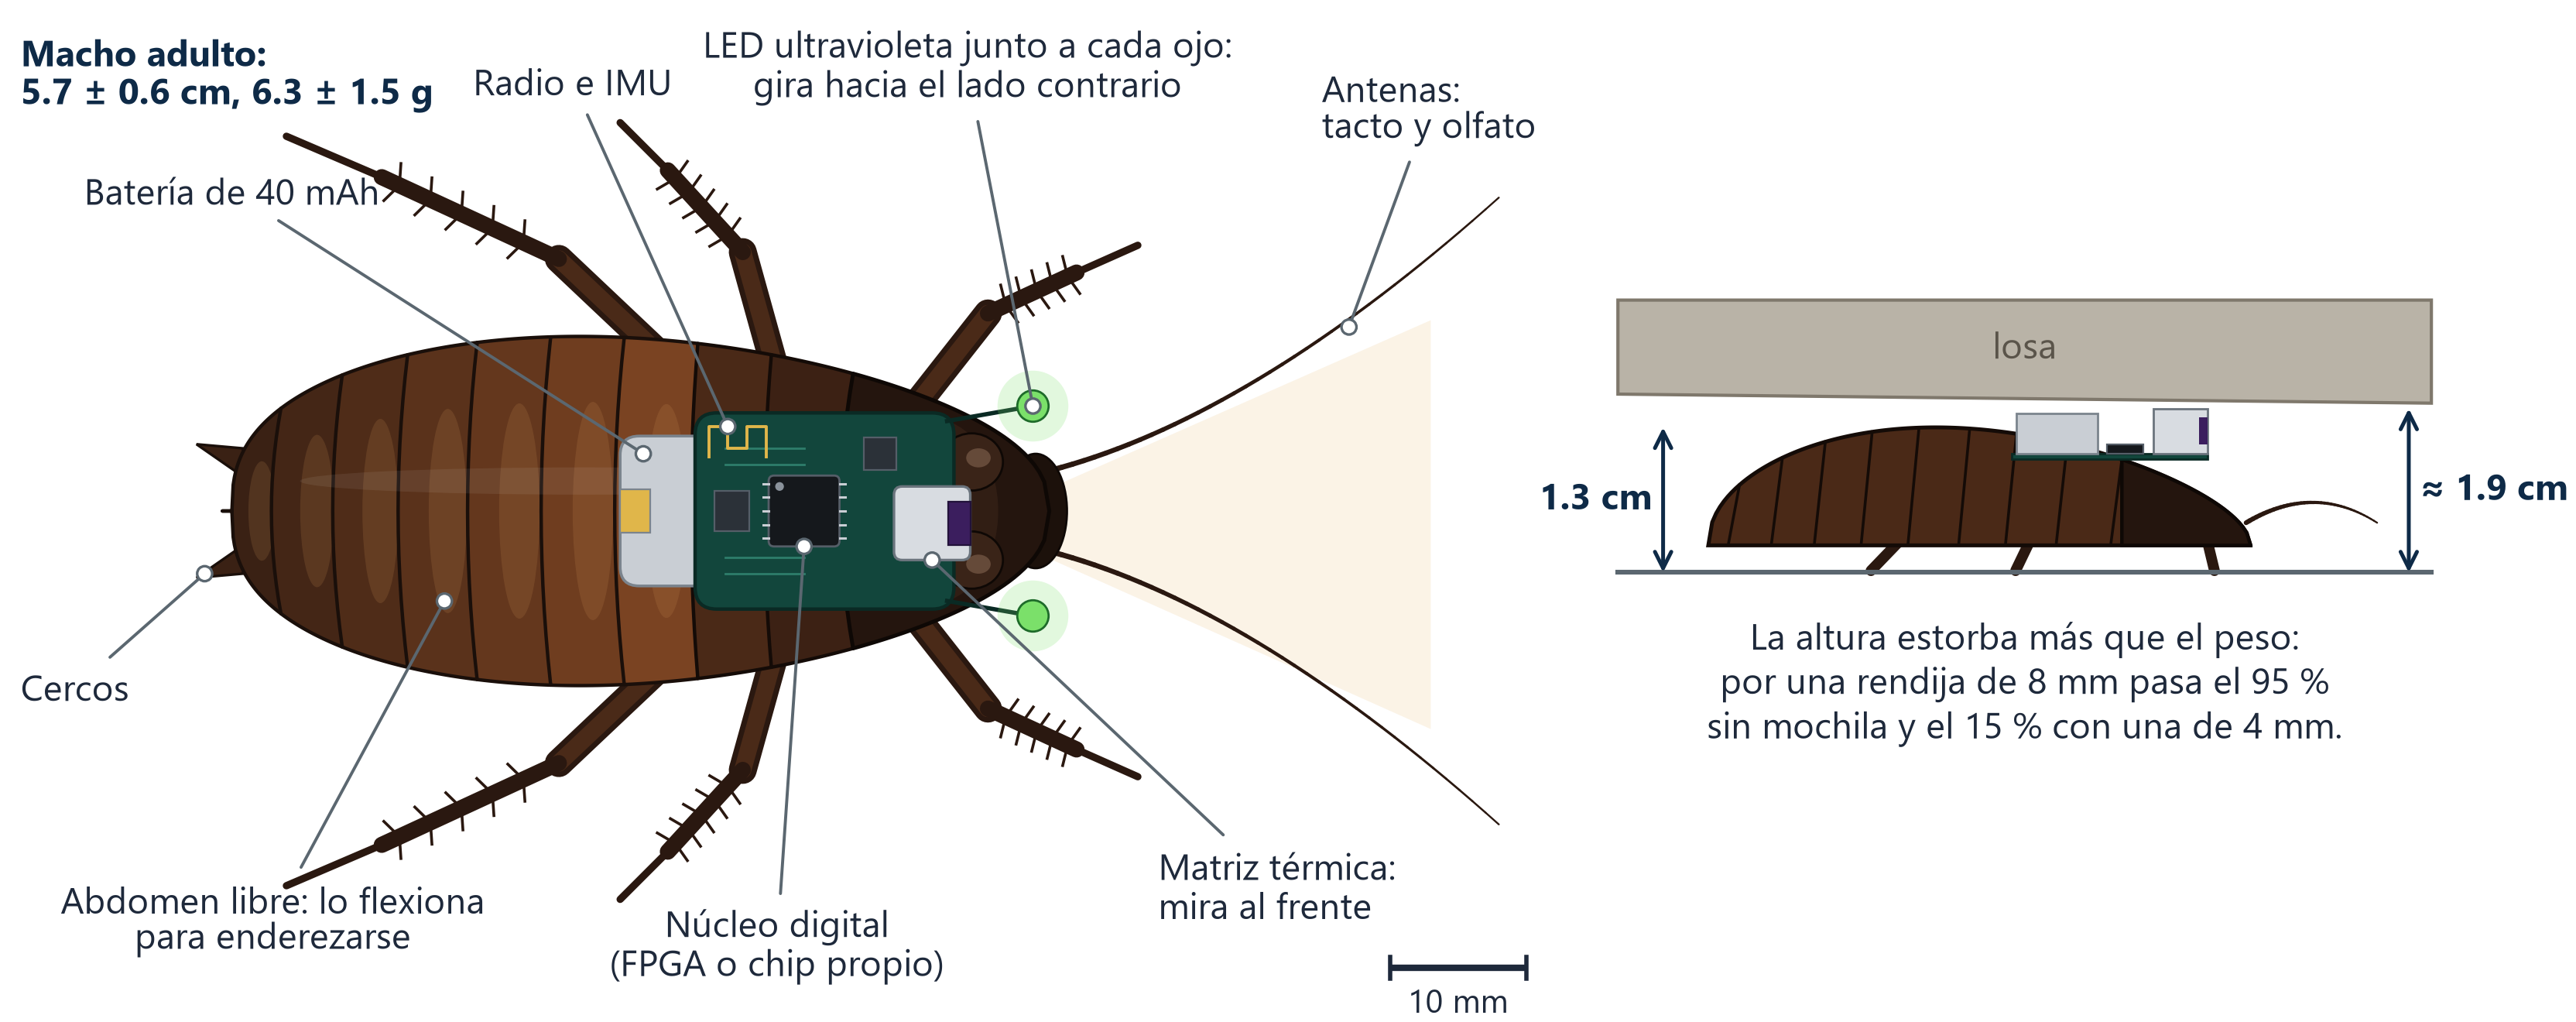
\includegraphics[width=\textwidth]{figs/insecto_mochila.png}
\caption{\Gp{} con la mochila, a escala. Dibujo esquemático propio; medidas de~\cite{tranngoc2023,li2019} y
paso por rendijas de~\cite{kai2026}.}
\label{fig:insecto}
\end{figure}

\begin{table}[H]
\centering\footnotesize
\caption{Capacidades de \Gp{} y lo que implican para la mochila.}
\label{tab:capacidades}
\rowcolors{2}{SoftGray}{white}
\begin{tabularx}{\textwidth}{@{}>{\bfseries\raggedright\arraybackslash}p{2.6cm} >{\raggedright\arraybackslash}p{5.4cm} >{\raggedright\arraybackslash}X@{}}
\toprule
\rowcolor{TableHead} Capacidad & Dato publicado & Consecuencia de diseño \\
\midrule
Masa y tamaño & Macho adulto: $6.32\pm1.5$~g y $5.7\pm0.6$~cm~\cite{tranngoc2023}; 2.2~cm de ancho y 1.3~cm de alto~\cite{li2019} & La mochila se dimensiona para un animal de 6~g \\
Carga & Se cita un máximo de 15~g, pero con 15~g se detiene por completo~\cite{montagut2024}; con 4~g ya empeora el control~\cite{latif2012} & Meta de 2 a 3~g (30 a 45~\% de la masa corporal) \\
Altura & Rendija de 8~mm: pasa el 95~\% sin mochila y el 15~\% con una de 4~mm~\cite{kai2026} & Componentes uno junto a otro, no apilados \\
Velocidad & 1.9~cm/s en marcha natural~\cite{dirafzoon2017}; 3.7 a 5.0~cm/s guiada~\cite{tranngoc2024}; 3.3~cm/s sostenida 20~min~\cite{herreid1981} & El modelo usa 1.9~cm/s y 5~cm/s durante 4~s tras un estímulo \\
Pausas & Sin estímulo pasa quieta cerca del 60~\% del tiempo, con pausas de 37~s en promedio~\cite{dirafzoon2017} & La política debe reiniciar la marcha \\
Obstáculos & Trepa un escalón de 1.5~cm en 48 de 49 intentos; no trepa una pared lisa de 10~cm: la bordea~\cite{tranngoc2023} & La exploración sigue contornos \\
Enderezarse & 98~\% sin carga; 31 a 69~\% con mochila y hasta 82~\% con un diseño que lo facilita~\cite{li2019,montagut2024} & Mochila baja y ligera; no pegar nada rígido en el abdomen~\cite{kakei2022} \\
Temperatura & Actividad máxima cerca de 30~\textdegree C; a 34 y 38~\textdegree C pasa inmóvil más de la mitad del tiempo~\cite{gracidas2026} & Ventana de operación de 22 a 30~\textdegree C \\
Sentidos & Sigue paredes y huye de la luz; no huye del viento~\cite{mcgorry2014}; nada indica que busque personas & La detección es tarea de la electrónica \\
Energía & 5~mW en reposo y 17 a 31~mW caminando (cálculo propio a partir de~\cite{herreid1981}) & La locomoción la paga el insecto; la mochila solo alimenta sensores y radio \\
Resistencia & Al menos un mes sin comida ni agua~\cite{yoder1997}; vive de 2 a 5 años; no vuela ni muerde & Logística sencilla: se cría y se transporta sin cuidados especiales \\
\bottomrule
\end{tabularx}
\end{table}

\begin{figure}[H]
\centering
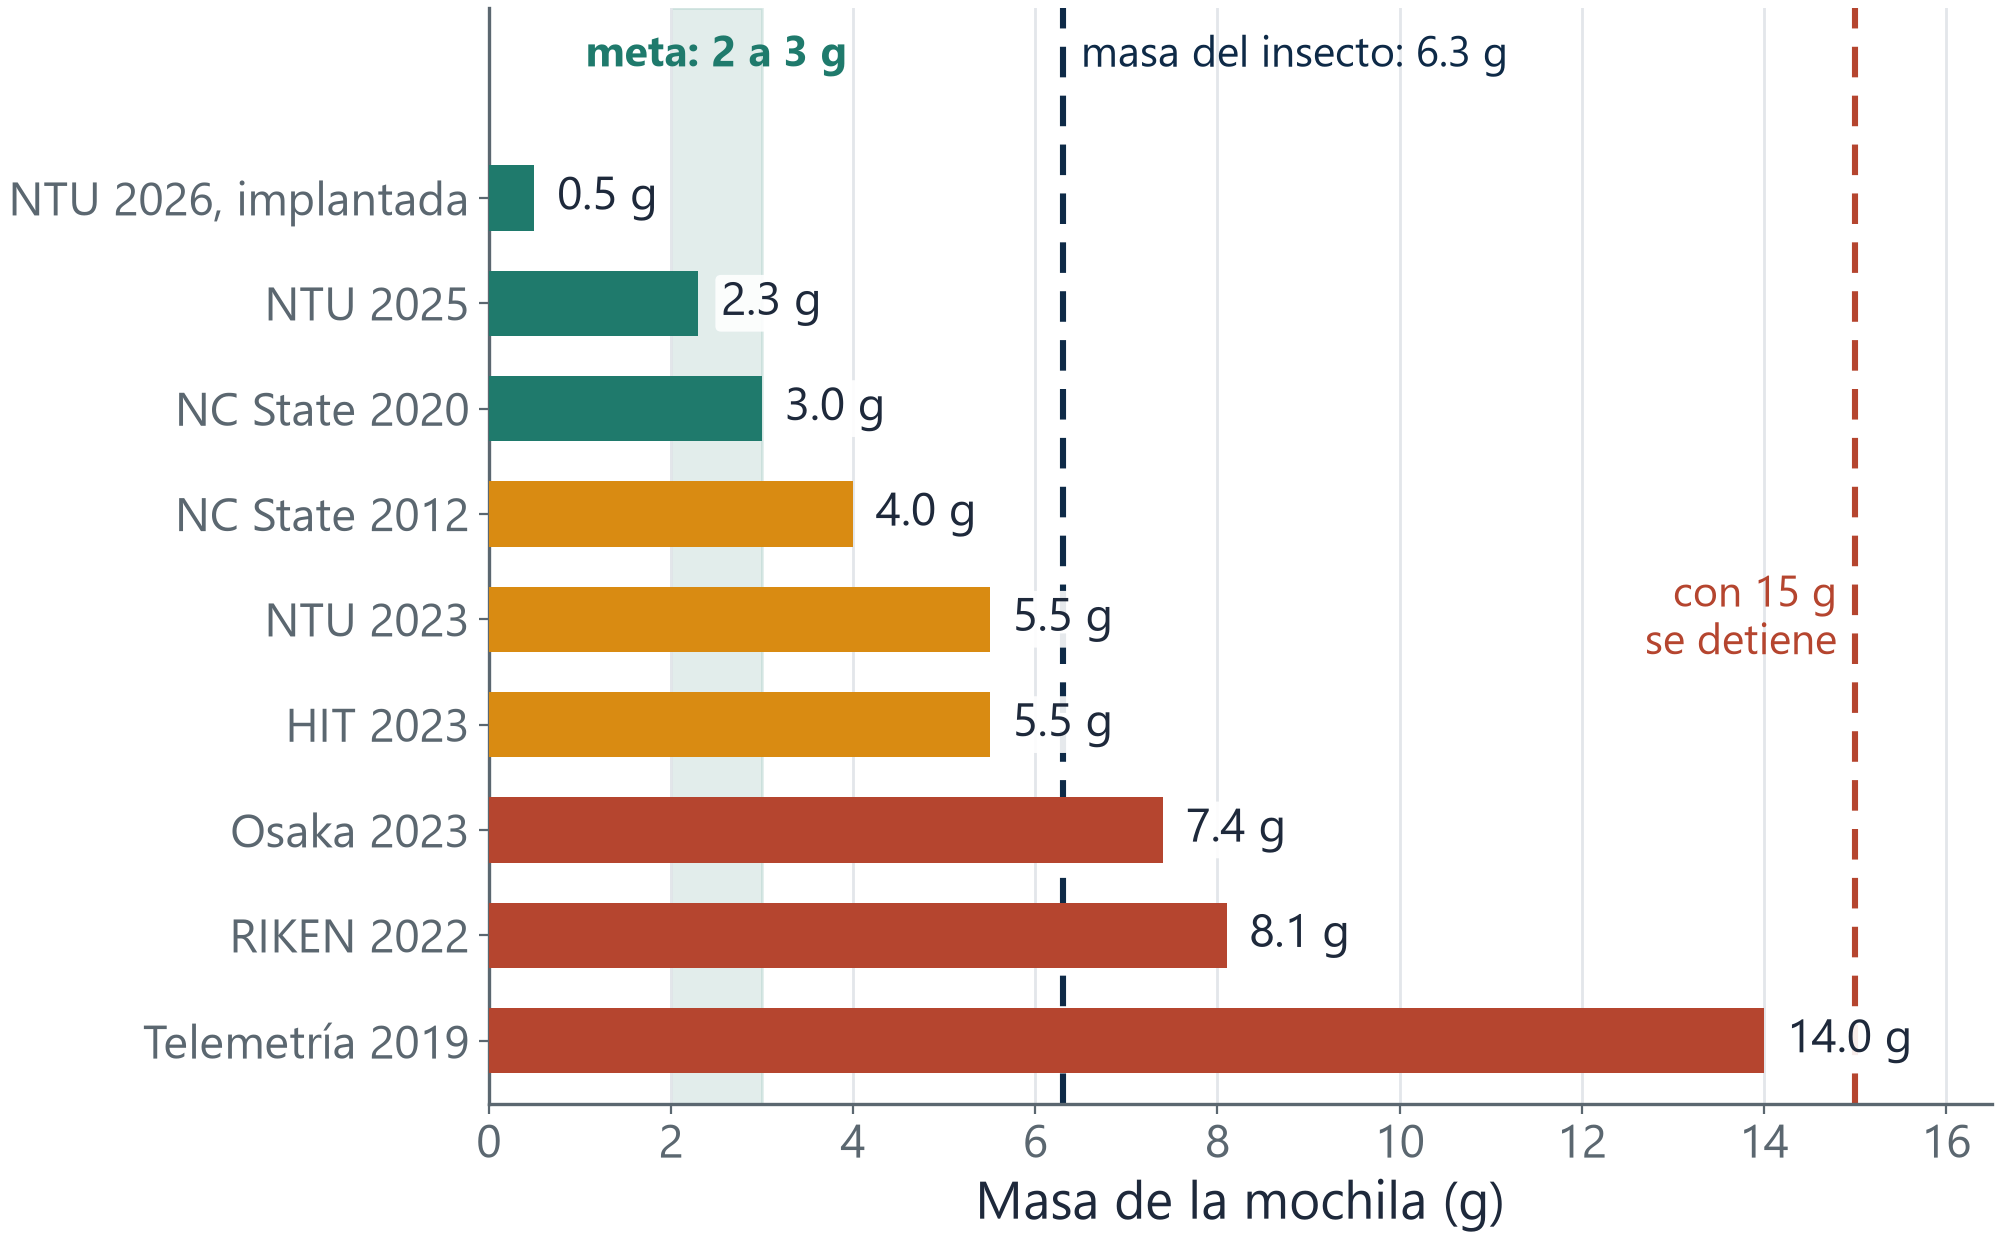
\includegraphics[width=0.78\textwidth]{figs/mochilas_publicadas.png}
\caption{Masa de las mochilas publicadas para esta especie. La tendencia es bajar masa y perfil:
el grupo de NTU pasó de 5.5~g en 2023 a 2.3~g en 2025 y a un controlador implantado de 0.5~g en 2026.}
\label{fig:mochilas}
\end{figure}

\subsection*{Supuestos iniciales que se corrigen}

La revisión obligó a cambiar cuatro cifras con las que arrancó el proyecto
(tabla~\ref{tab:correcciones}).

\begin{table}[H]
\centering\footnotesize
\caption{Supuestos de la propuesta inicial frente a la evidencia.}
\label{tab:correcciones}
\rowcolors{2}{SoftGray}{white}
\begin{tabularx}{\textwidth}{@{}>{\bfseries\raggedright\arraybackslash}p{3.1cm} >{\raggedright\arraybackslash}p{3.6cm} >{\raggedright\arraybackslash}X@{}}
\toprule
\rowcolor{TableHead} Supuesto inicial & Valor inicial & Evidencia y valor adoptado \\
\midrule
Carga útil & 15~g sin afectar la marcha & 15~g es el punto en que el insecto se detiene~\cite{montagut2024}. Se adoptan 2 a 3~g \\
Velocidad & 0.3~m/s & Lo medido va de 3 a 9~cm/s; 0.3~m/s corresponde a otras especies. Se adoptan 1.9 y 5~cm/s \\
Detección térmica & Umbral fijo de 35.5 a 38.5~\textdegree C & Es temperatura central; la piel expuesta está entre 27 y 35~\textdegree C y el sensor promedia su campo de visión. Se cuenta píxeles calientes sobre el fondo \\
Tamaño del circuito & Menos de 60 celdas & La síntesis del núcleo completo da 224 registros y 477 elementos lógicos \\
\bottomrule
\end{tabularx}
\end{table}
